\documentclass[letterpaper, 12pt]{report}
\usepackage{fullpage}
\usepackage{chronology}
\usepackage{graphicx}
\usepackage[normalem]{ulem}
\usepackage{csquotes}
\usepackage{indentfirst}
\usepackage{caption}

% Title Page
\title{Final Writing Portfolio: The Use of Cellphones in the Student Worker Environment}
\author{Huyanh Hoang\\ Informatics 162W Section 3}
\date{\today}


\begin{document}
\maketitle
\tableofcontents

\pagebreak
\section*{Acknowledgements}
\noindent Many thanks to the UCI Student Center for providing the site of study. Thanks to the people that willingly let us observe them. Thanks to our team that helped contribute to the research notes. Lastly, thanks to Kendi Rosas Goss for granting access to the observation site. For more information, contact kendi@uci.edu.

\part{Executive Summary}
\section{Introduction}
This document summarizes the results found in the paper titled \textit{The Usage of Cellphones in the Student Worker Environment}. The purpose of the study is to understand the nuances and implications of students being able to use their smartphone on shift in the university level student work environment.

\section{Conclusion (Summary of Findings)}
During breaks, student workers tended to sit together in a circle but not talk to one another. In a conversation between two students, we saw that the students talked about why they enjoyed working at the Student Center. They explained that they like it because of the people aspect, although when these workers were grouped up, they were on their cell phones.\\

Students during work would also have a tendency to use their cellphones. This usage would affect the other workers, as the time spent on cellphones could be use to help set up other equipment.\\

On certain shifts, students who used their cellphones also would talk to their coworkers. The more people were interacting with each other, the less likely they were to use their phones.

\section{Methods}
This research consists of 10 hours of qualitative ethnographic observation throughout the course of 10 weeks from January to March.\\

The observation was done in a different room of the Student Center for 1 to 2 hours per observation. We took field notes on three night operations shifts, two game room shifts, and one meeting. We leveraged all of our data with the literary examples to find out why and how the use of smartphones affect the efficiency of workflows. To know this, we observed what the workers are doing on their smartphones and recorded the applications they used.


\section{Recommendations}
We recommend investigating further and asking questions relating to the correlation between the level of freedom in the workplace and overall job satisfaction. The sample size and focus group for this observation is also limited because of the 10 hours of observation. Other universities will need to be considered, as well as different types of work organizations in order to generalize these findings. Besides ethnographic observation, more qualitative studies will need to be done such as interviews with student workers and their managers. Answering these questions may help understand if smartphones actually negatively affect student worker interactions and if this can be generalized to other organizations and workers.

\section*{For More Information}
Huyanh Hoang, Undergraduate in the Department of Informatics - University of California, Irvine. IN4MATX 162W, Bietz. huyanhh@uci.edu.


\part{Project Proposal}
\section{Introduction/Summary}

The site that our team chose to study is the UCI Student Events Center. We are primarily interested in finding out the workflows of student worker communication and how tasks are delegated to one another. We will observe and see if these systems are satisfactory, and hope to achieve an in depth understanding about these particular systems. Potential obstacles include bias and trust. The cost will come out to 0 dollars: 0 interviews, and 10 hours of observation time.

\section{Context}

The Student Center provides venues for events, available to clubs, business, and other professional/nonprofessional organizations that might or might not be from UCI. The size of the venues can range from a small room for 30 people to a large room for 300 people. The Student Center also provides services such as Zot Zone, where students can rent video games or pool tables for as long as they want, Courtyard Study Lounge, a study area with 15 rooms for students to reserve, and the OIT lounge, which is the room where UCI provides public PCs and Macs for students to use.\\

From our first observation, the team went around 9:00pm and observed a night operations shift. On this day, the workers, known as the crew, had a task list seemed to be set by the manager of that shift. The work was delegated by a Building Lead (BL). The BL assigned mini tasks to a section of the crew, around 2 people, and took 3 other ops members with her to the Newkirk Alumni Center building in Mesa Court. The observation team followed the crew going to the Newkirk Alumni Center. There, according to the diagram presented in the daily task list, the crew set up two rooms with chairs totaling around 200.\\

For each shift, the crew has around 5-6 people, there is one BL, and there is one manager. The crew uses radio communication to send requests and do checkups. The managers  seem to report to higher authority, but we do not know yet about the actual chain of command. We can be sure though, that there is a main director and a board of directors under that main director.

\section{Project Plan}

\subsection{Goals}
The goal of the project is to understand channels between student employees and other communications among the various levels.

\subsection{Plan}
The plan is to observe communications between all the various levels in the Student Center operations hierarchy. We will observe one student and how he or she communicates with the student's coworkers. Operations interactions will be studied in detail to find out about the efficiency of communications with respect to the work that the employees do. The type of notes that will be taken consist of mainly qualitative observations.

\subsection{Location}
There are four sub-sites of observation: in the Student Center office, in Courtyard Study Lounge, in Zot Zone, and in the various rooms inside the Student Center during event setup and coordination. The times of observation will be distributed evenly throughout each sub-site. The Student Center office will be observed at the same times as the other three sites, since it acts as a base of operations hub for the employees.

\subsection{Time}

Since the schedules of the student employees vary, and we are going to follow one student, the times of observation will vary. To make the most out of the 10 hours of observation, the observations will take place in the morning, during the middle of the day, at night, on weekdays, and on the weekends.

\subsubsection*{Timeline by Week for Planned Observations}

\begin{chronology}[1]{2}{10}{\textwidth}[\textwidth]
	\event{3}{Weekday (Student Center)}
	\event{4}{Weekday (Zot Zone)}
	\event{5}{Weekday (Courtyard Study Lounge)}
	\event{6}{Weekend (Student Center)}
	\event{7}{Weekend (Zot Zone)}
	\event[8]{8.5}{Weekend (Courtyard Study Lounge)}
	\event[8.5]{9}{Weekend (Courtyard Study Lounge)}
	\event[9]{9.5}{Weekday (Student Center)}
	\event[9.5]{10}{Weekday (Student Center)}
\end{chronology}

Each week will consist of one hour of observation. Two observations are done for week 8 and week 9 because finals are coming up for the students, and we predict behavior might be different.

\subsubsection{Deliverables}

\noindent Project Proposal\hfill Jan 25 at 2:00pm\\
Project Proposal Critique\hfill Jan 28 at  at 2:00pm\\
Case Study\hfill Feb 8  at 2:00pm\\
Case Study Critique\hfill Feb 11 at 2:00pm\\
Progress Report\hfill Feb 18 at 2:00pm\\
Progress Report Critique\hfill Feb 18 at 2:00pm\\
Research Paper\hfill Feb 29 at 2:00pm\\
Research Paper Critiques\hfill Mar 3 at 2:00pm\\
Executive Summary\hfill Mar 7 at 2:00pm\\
Executive Summary Critique\hfill Mar 10 at 2:00pm\\
Writing Portfolio\hfill Mar 17 at 5:00pm


\section{Resources and Risks}

The site requires us to have approval to observe the student workers. The Student Center is a quasi-public type site, so as students we already have access. We might also need a schedule of employee work times, so we can plan our schedule around that. We will need to invest 10 hours into observation. Some challenges include confidentiality, trust, information overload, sampling bias, and interpretive bias. Trust and confidentiality issues can be resolved by communicating well with the employees. We will explain what we are doing with the data, enough for them to understand our sincere intentions. The attire worn during observation will be similar to the uniforms of the employees, so they will not be too intimidated: t-shirt and casual pants. Errors and biases can be diminished by routinely studying the same type of people and keeping variables to a minimum. Seemingly irregular occurrences will show themselves again if they are norms Interpretive bias can be minimized by observing as a team; by comparing notes afterwards and having discussions, interpretations can be uniform throughout the project.

\section{Significance}

This is an important project because my teammates and I are interested in applying for a job at the Student Center in the future. By understanding the work culture of the Student Center, we can better understand if this job suits us as UCI students. We are curious about the employee satisfaction and what kind of equity is given to student employees. We as students are constantly involved in the events at the Student Center such as the career fair, so by understanding what goes on in the background, we will also learn to appreciate the hard work that goes into the event set up process.\\

In terms of organization of structure, it is interesting to get insight on how a top down structure like the Student Center works because as students majoring in computer science, we can compare this structure to our future work in corporations, and see how interactions play a role in overall efficiency. At the end of the project, we will understand another type of environment that we might be interested in working in.

%Really light on information systems here. How did the crew get the order? Where did the building lead get them from? Tell me more about the information on the diagram. How did it get there? Why?

\part{Case Study}
\section{Introduction \& Context}
%Describe the organization in relation to the case you will focus on
This study focuses on a two hour on-site informal observation done on Febuary 7, 2016 from 7:00pm to 9:00pm. The study will describe the workflows and behaviors of the L1.a operations crew members. These workers are the bottom level of the organizational structure, and they are the positions that a worker will first start off as upon joining the organization. Workers can be promoted to L1.b, L2, L3, and finally L4. All workers from L1.a to L4 must be students. Dress code of basic crew members is same up to the L4. Student Managers: Dark blue t-shirt with the Student Center logo. Duties that L1.a student workers are expected to do include cleaning tables, carrying tables and chairs from closets to demount and reposition, handling A/V equipment, taking out trash in rooms, and working with their L3 crew leads in the morning and L2 building lead at night. They have the least responsibility out of all of the roles, and work smaller shifts than the others. All of the crew are responsible for setting up and understanding layouts of all the rooms: Doheney Beach, Emerald Bay, Moss Cove, Woods Cove, Newport Beach, Pacific Ballroom, and Crescent Bay.\\

Each shift, the building lead (BL) has a task list that is typed up and handed down by either the normal manager on duty or L4 student manager on duty. The building lead has the responsibility of making sure the tasks for a particular night are done and the rooms are setup properly for upcoming events. If needed, the building lead will manually walk to each room at the end of the night to do quality assurance tests. For the task list, each task contains a diagram of a different setup for each room. Each diagram depicts the chairs, tables, and other items that may go in the setup, and the amount of items are determined by the amount of people who are attending that event.

\section{Case: Pacific Ballroom Event Setup}
\subsection{Details}
On this shift, the current task consisted of an event setup in Pacific Ballroom of the Student Center for February 9. The crew, consisting of 10 workers, mainly followed the orders of the building lead and set up the room as it was in Figure \ref{fig:ballroom1}. Noted by the diagram, the setup consisted of 18 round tables, 110 chairs, commissioned by the Physical Sciences department for the ``Physical Science Breakfast Lecture Series." At 7, when one worker walked in the room, the rest of the crew was already setting up tables and chairs and putting the ones from the day before away. The worker, Marvin, walked up to one of the other crew members and asked ``okay, what are we doing right now?" It was a very casual manner of speech, and the other worker, Tim, laughed at Marvin because Marvin was eating a sandwich when he walked in: ``dude, I didn't even know you were working cause you were eating a sandwich!" For the next 30 minutes, the crew stacked chairs and moved tables without interaction. Every couple minutes, the workers would go to the table where Ivy placed her clipboard, which contained the tasks for the night, and compare the diagram to the tables that they just put down.\\

The work pace slowed down afterwards, when most of the chairs were put away. At that point, some of the crew took out their phones while others worked on putting away the remaining chairs. Ivy, the building lead for that day, shouts from the other side of the room: ``Guys, can you get the tables?" Immediately, everybody from the other side stood up and start walking towards the closet to grab big, rectangular tables to adhere to the room setup. Ivy and the rest of the crew has a radio with them, but Ivy does not to use it.\\

After the tables were placed, they were inspected for alignment. The tables were required to be almost the same as the diagram's in terms of spacing. The inspection required two people: one to shift the tables and one to look from a distance to estimate the alignment.\\

Once that work was finished, at 8:40 the members were allowed a ten minute break. During the break, the building lead asked three workers to come with her, and chose three at random. They immediately got off their break and followed the lead to a different room.
\subsection{Important Features}
When the crew was working, a worker, Ramiro, had connected his phone to the aux speaker and was playing music. The music was from his personal playlist, consisting of rap, hip-hop, and R\&B. The workers did not talk to each other much, and spoken words were normally requests from the Building Lead.\\

The workers do not seem to be briefed about exact specifications when they get on shift. The BL delegates the items on the diagram verbally to the workers. When Ivy called across the room for the crew to carry out the tables, without hesitation, went to the closet to take out the table, and only when they set it half of them down did they actually look at the diagram to see if they needed more tables or where the tables were supposed to be placed.\\

Both the workers and the building lead do the setup. Ivy delegates the tasks and tells everyone to do a specific task, i.e. getting tables, but she goes and gets tables as well.\\

On the break and on the completion of each task, the majority of the crew took out their phones and sat in a circle. No one talked to each other. At one point Marvin talked to Ramiro. They had not met before, so they introduced themselves. Ramiro asked ``How do you like working here?" and Marvin responded with ``It's good. The hours are terrible, but the people are really cool. It's the most social job you can have on campus."\\

Another interesting feature was the way the crew relaxed on their break. Some workers sat on a table; some sat backwards in a chair, and one person was even sprawled on her own table, falling asleep.

\section{Discussion}
%Why is this an interesting example?
Today's generation is highlighted by the copious amounts of information technology and its usage. People are social, yet unsocial at the same time. By the casualness of their interactions, the crew seems to appreciate one another as friends, but they do not talk as much as one would think of in a normal friendship. The casual environment set by the workplace facilitates such behavior. In other settings, such as restaurants and coffee shops, management would not allow workers to play their personal music.\\

This casualness influences other behaviors as well, as exemplified by the manner in which they take their breaks. They go on their phones and sit in a circle, a habit of adolescents and young adults today when they socialize. It seems ironic that Ramiro and Marvin agree that the best part of their job is the people. As the ``most social job you can have on campus," perhaps there is more to just the interactions we observed.\\

The Student Center, which employs student workers, seems to have a culture that mirrors that of normal UCI school life. Norms, values, and assumptions are almost ``imported" into Student Center life, in a way. As the workplace does not enforce rules of strict dress code or no personal music, although workers take their job seriously, they tend to exhibit behaviors of any typical college student at the workplace. In other workplaces, workers might constantly be doing a task, as opposed to the Student Center. The lax rules defined by the Student Center result in a work culture that is very casual and easygoing.\\

The Student Center culture affects the information systems in a variety of ways. Since the workplace is made up of students, distribution of work is very decentralized. The student manager or manager hands the tasks down to workers in the lower levels, and then from there the workers all have the same information. Even though the building lead has a higher position, the building lead's role is simply to make sure that the task list is done. The L1.a workers do not necessarily need to get the tasks directly from the building lead, as we observed that they only needed to look at the diagram set-up to understand their work. Another effect of the culture is the way that the building lead communicates tasks to the team. When Ivy needed the L1.a workers to get tables, she shouts from the other side of the room. She does not use her radio even though she was on the other side of the room. The room at the time was going to be set-up for 100 people, so there was around 200 feet of distance between her and the L1.a workers. As peers to each other, both the building lead and the L1.a workers communicate in a very informal manner even though they are doing professional work.\\

Communication with any of the upper levels of the organization has not been studied yet and is beyond the scope of this study, so we do not yet have a complete grasp of patterns of interaction. We can understand, however, that workers are very casual with each other, whether it be building lead to crew or crew to crew. Languages and themes do exist, of course, but more observation will need to be done to notice obvious patterns.

\begin{figure}
	\section{Figures}
	\centering
	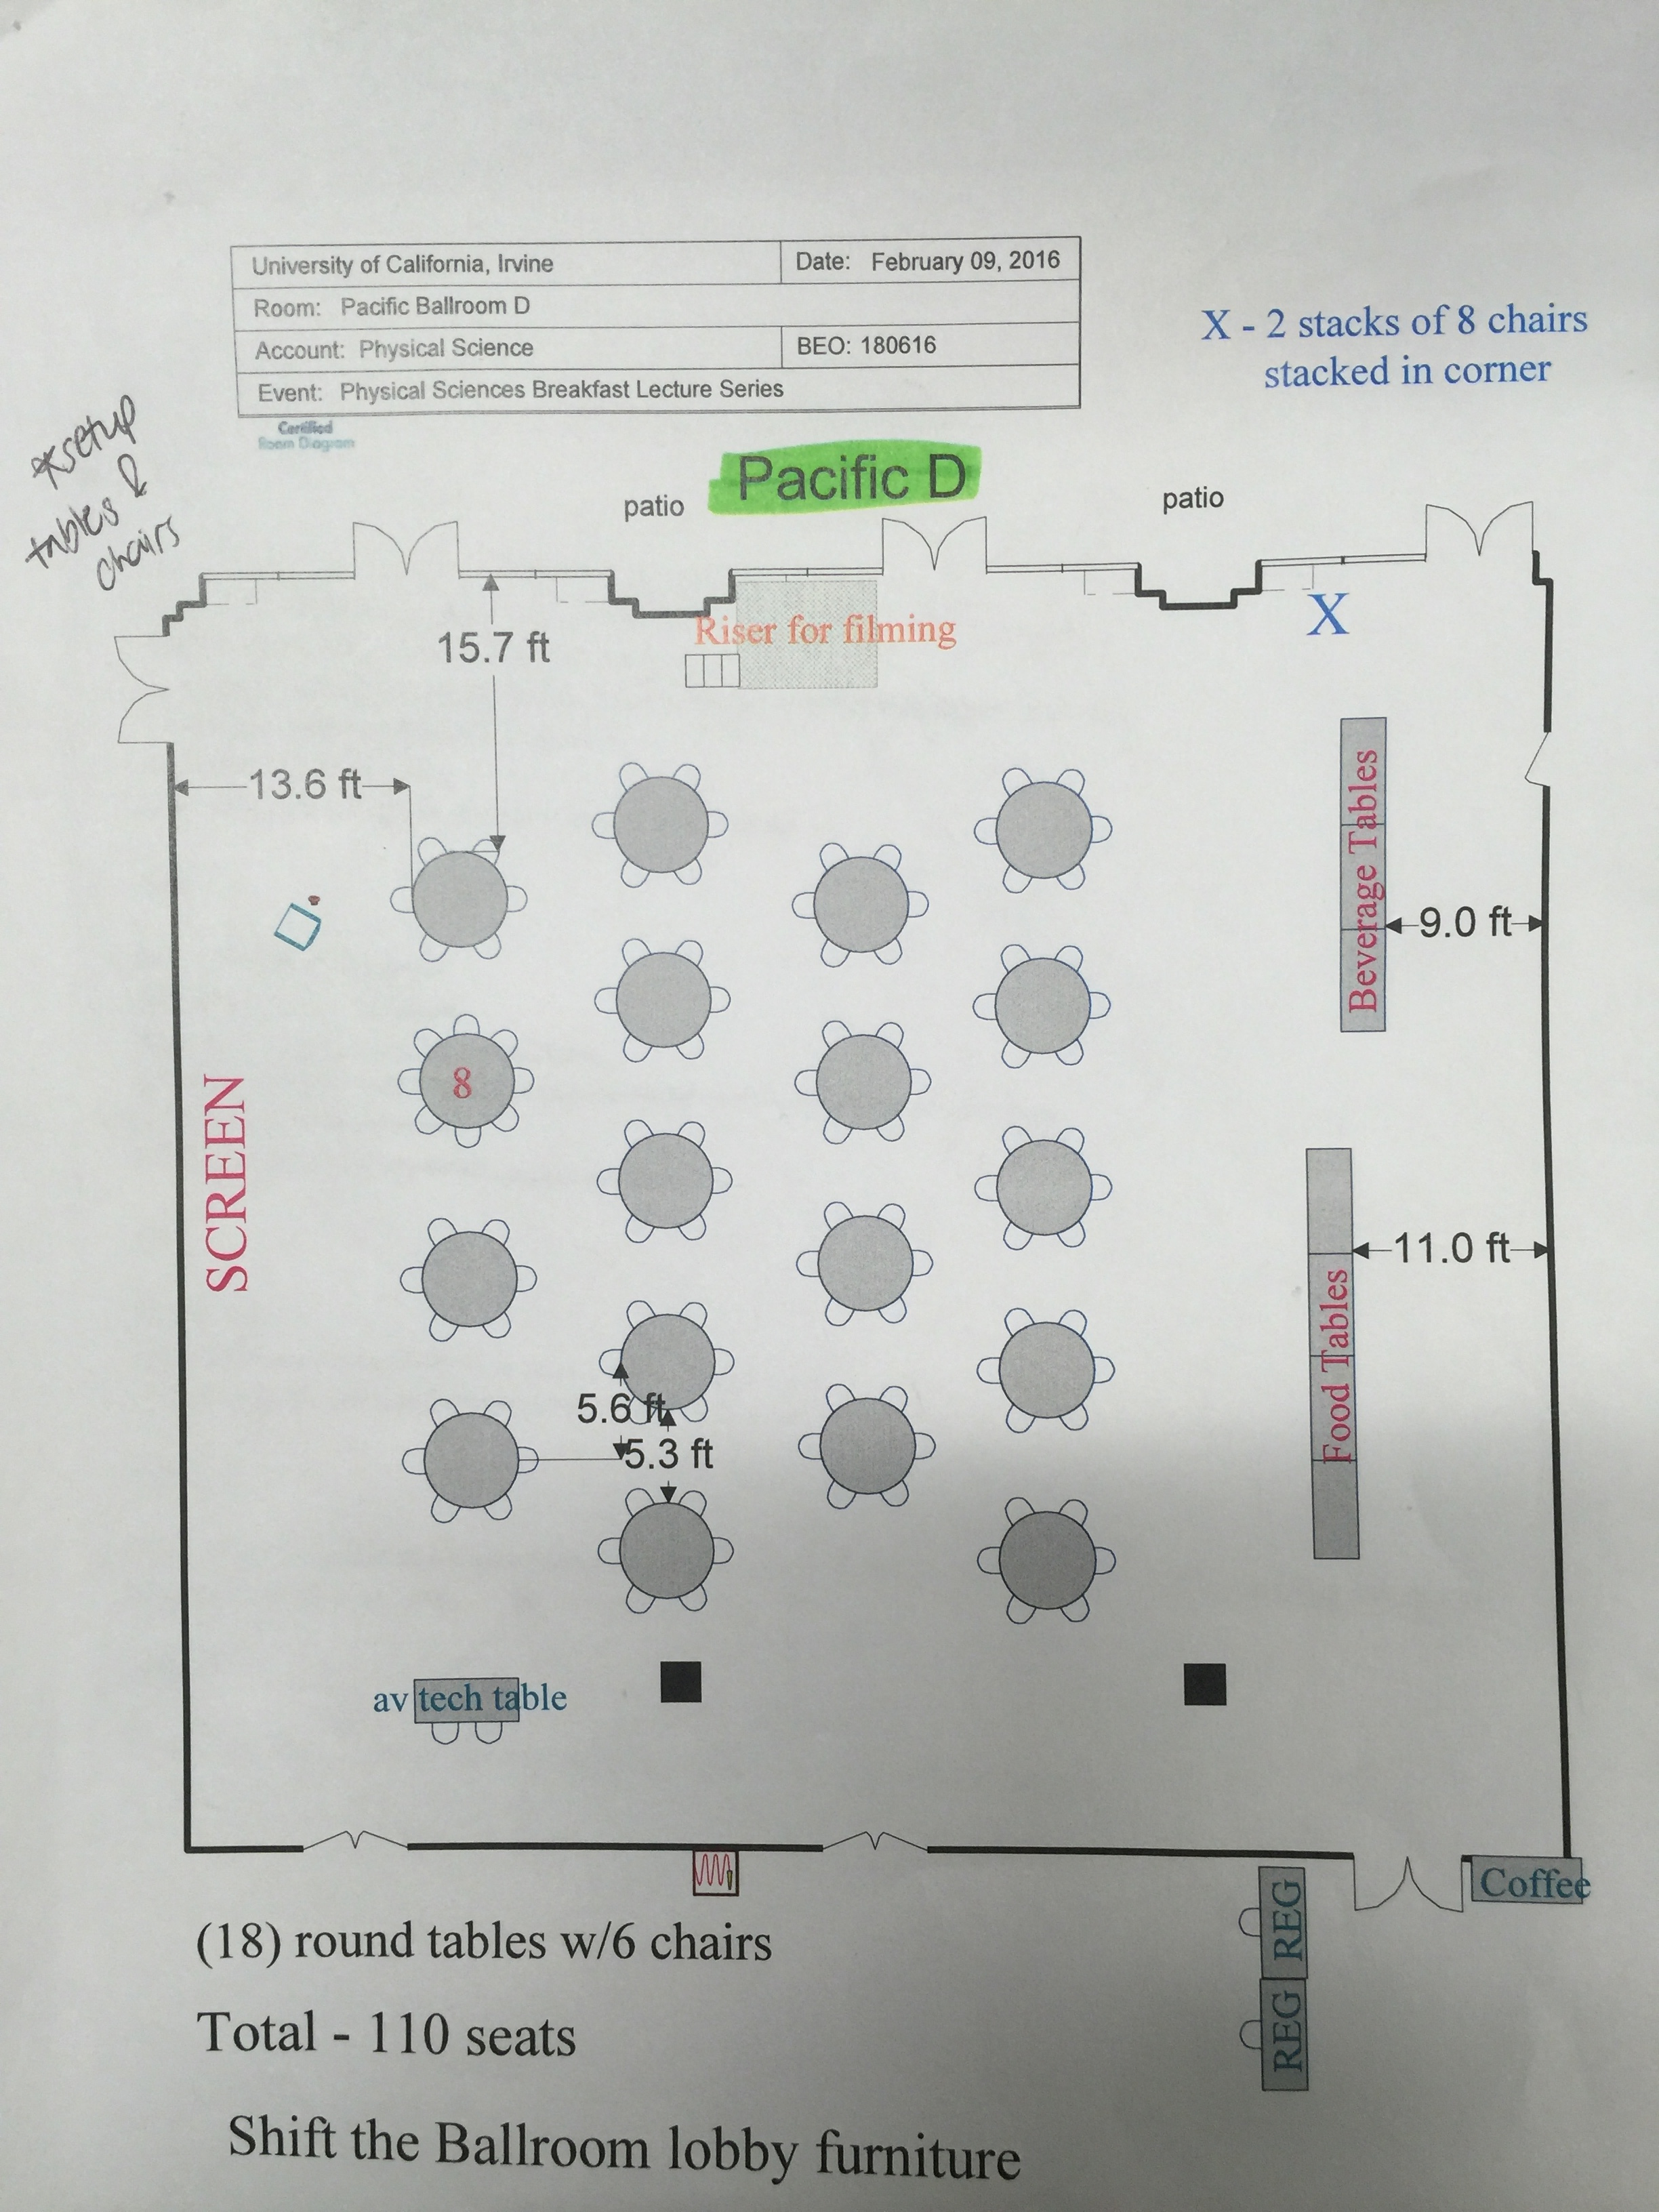
\includegraphics[width=15cm]{diagram.jpg}
	\caption{Pacific Ballroom D Diagram}
	\label{fig:ballroom1}
\end{figure}


\part{Progress Report}
	\section{Background}
	The Student Center provides venues for events, available to clubs, business, and other professional/nonprofessional organizations that might or might not be from UCI. The Student Center work consists of event set up throughout the Student Center and management of the Zot Zone and the Visitor Center. The project that will be done is an observation of the processes of the Student Center and understand the roles of information systems in various levels of the Student Center operations crew.\\
	
	In the timeline of observation, the original plan was to have an hour of observation a week, with double the amount near the last two weeks of the quarter.
	
	\begin{chronology}[1]{2}{10}{\textwidth}[\textwidth]
		\event{3}{Weekday (Student Center)}
		\event{4}{Weekday (Zot Zone)}
		\event{5}{\sout{Weekday (Courtyard Study Lounge)}}
		\event{6}{\sout{Weekend (Student Center)}}
		\event{7}{\sout{Weekend (Zot Zone)}}
		\event{8.3}{\sout{Weekend (Courtyard Study Lounge)}}
		\event{8.7}{\sout{Weekend (Courtyard Study Lounge)}}
		\event{9.3}{Weekday (Student Center)}
		\event{9.7}{Weekday (Student Center)}
	\end{chronology}
	
	It has been come to a decision that the schedule will be modified, as events have come up that impeded the ability to come observe. One important thing to note is that the Student Center Courtyard Study Lounge is no longer monitored by students. The system is now run exclusively online. Therefore, future observations that were originally the Student Center will be moved to the Visitor Center. Another problem includes personal schedules and Student Center scheduling conflicting. The new tentative schedule will be modified as follows:
	
	\begin{chronology}[1]{2}{10}{\textwidth}[\textwidth]
		\event{3}{Weekday (Student Center)}
		\event{4}{Weekday (Zot Zone)}
		\event{7}{Weekday(Student Center)}
		\event{7.6}{Weekday (Zot Zone)}
		\event{7.9}{Weekend (Student Center)}
		\event{8.5}{Weekend (Visitor Center)}
		\event{9}{Weekday (Visitor Center)}
		\event{9.6}{Weekday (Student Center)}
		\event{9.9}{Weekday (Student Center)}
	\end{chronology}
	
	The new observations will be pushed as close as possible to each other near the end of week 7 because it will be right before students prepare for finals, and so it will be the last time seeing mid-quarter behaviors.
	
	\section{Achievements}
	%i think the TA will want a table here for next time
	So far, we have done three observations and and case study of one of the Student Center night observations. The observations have been going as expected. Field notes have been recorded for all three. The last Zot Zone shift that was observed was actually a special event, and workers exhibited alternative behaviors that we would not see in a normal event. The Zot Zone during the weekday will have to be observed again as a result. Otherwise, there have been no special exceptions for the Student Center, so they will be observed as planned.
	
	Below is a table of the milestones that have been achieved so far:
	\begin{table}[ht]
		\centering
		\caption*{Table 1: Milestones and Status}
		\begin{tabular}{l l}
			\hline\hline
			Milestones & Status\\
			\hline
			Project Proposal&Completed \\
			Case Study&Completed \\
			Progress Report&In Progress\\
			\hline
		\end{tabular}
		
	\end{table}
	
	These milestones have been completed and are awaiting critique. Once these deliverables are revised they will be added to the final portfolio.
	
	\section{Challenges}
	Not many challenges have arisen aside from the fact that the Courtyard Study Lounge is no longer monitored by students. This led to a need to reschedule with the client so that future Courtyard Study Center observations will be have to be somewhere else. The Visitor Center has been chosen for that matter.
	\section{Remaining Research}
	The rest of the observation has to be done within the next three weeks. Since the scope of the project is more narrow than that of most projects, there is more room for breather, so observation techniques will not have to be modified. The plan of action still follows: observe the information systems of student workers and the methods in which they communicate. Future work to be done includes studying the higher levels workers more carefully and communications with their managers.
	
	\begin{table}[ht]
		\centering
		\caption*{Table 2: Future Deliverables and Due Dates}
		\begin{tabular}{l l}
			\hline \hline
			Deliverables&Due Dates\\
			\hline
			Research Paper&Feb 29 at 2:00pm\\
			Executive Summary& Mar 7 at 2:00pm\\
			Writing Portfolio& Mar 17 at 5:00pm\\
			\hline
		\end{tabular}
	\end{table}
	
	For the research paper, we have not formed a specific research question yet. Therefore, we will be looking for interesting things around the methods that the workers use communicate.
	
	\section{Reflection}
	There is a high chance I will meet my objectives on the intended schedule, around week 10. So far the original objectives will remain the same, unless more interesting points are bought up in the future. The main challenges that I will face will mainly be schedule conflicts, because as a student I also will have finals to study for and will not be able to research for the particular days that I schedule because of assignments. If so, the observation days will only pushed back with of a buffer of maximum two days. I will still be able to complete all 10 hours.

% Title Page

\part{Research Paper: The Use of Cellphones in the Student Worker Environment}


%https://www.elon.edu/docs/e-web/academics/communications/research/vol6no1/02DragoEJSpring15.pdf
	
	\section{Introduction}
	
	The objective of this research is to thoroughly examine the system of workflows of the student workers and understand the role of smartphones in influencing the university work environment. We will do an analysis to actually find out if these communications improve the workflows of the systems or if it hinders these systems. We will also put the impacts of technology usage in a broader perspective.\\
		
	We will be using the literature reviews below to support any argument made about the implications of using smartphones in the Student Center environment.\\
	
	The Student Center provides venues for events, available to clubs, business, and other on-campus and off-campus organizations. The size of the venues can range from a small room for 30 people to a large room for 1000 people. The Student Center also provides services such as the Bean Zone, where students can rent video games or pool tables for as long as they want, and the computer lounge.\\
	
	We will be examining the workflows and behaviors of the tier D operations crew members. These workers are the bottom level of the organizational structure, and are the positions that a student will first start off as upon joining the organization. Workers can be promoted to tier D2., C, B, and finally A. All workers from tier D to tier A must be students. Duties that tier D student workers are expected to do include cleaning tables, carrying tables and chairs from closets to demount and reposition, handling A/V equipment, taking out trash in rooms, and working with their crew leads in the morning and building lead (BL) at night. The workers all carry radios and use them to communicate tasks. The tiers C through A have responsibilities such as delegating tasks on the task list and doing quality assurance checks on rooms that are about to be used for upcoming events. All of the crew are responsible for setting up and understanding layouts of all the rooms of the Student Center.\\

	\section{Literature Review}
	\subsection{\textit{The Effect of Technology on Face-to-Face Communication}}
	The article explains about how the advancements in technology affect the way individuals communicate. Through field observations and an online survey, Drago (p. 14, 2015) determined "the level of engagement individuals have with their cell phones, other technologies and with each other in face-to-face communication." The research concluded that technology decreases the quality of face-to-face communication as well as the overall amount. Even if there were people around and the user was aware, it would not stop the user from still using the mobile devices. Questions arise such as "will employees be less able to communicate with their employers and, therefore, less able to succeed in the workface?" and "will the new skills developed through hours of cell phone use and texting result in a workforce that is more nimble and more qualified to multi-talk?"(Drago, p.17, 2015). Even if these questions are unpredictable, it is important to understand that human interaction is not what it was before.\\
	
	We will keep in mind that student workers in our observations might have similar characteristics to that of the subjects studied in this article. Both groups have a similar demographic, as they are undergraduate university students, and while this research was only done on 100 students, the results cannot be generalizable. Because of the demographic similarities we can make more informed hypotheses about the workers of the Student Center, however. We can refer to this article for trends and try to understand why even when being in the physical presence of others, users will stay on their phones.
	
	\subsection{\textit{Smartphones: Fulfilling the Need for Immediacy in Everyday Life, but at What Cost?}}
	This article explains the attitudes that college students have towards smartphones. Because smartphones provide immediacy and let the user stay "in the loop," users feel compelled go on their phone to check social media more often even when they know that they did not get any notifications. Young adults expressed concern about using their smartphone too much yet they still felt that they needed to rely on using it. The possibility of formed addiction is noted by this article. This addiction may erode away intimacy, a ``critical aspect of relationships"(Lindquist, 2014). Intimacy, according to the author, is developed primarily through honesty and boundaries are made permeable through verbal and written communications. It concludes to say that the negative effects outweigh the positive ones.\\
	
	It seems as communication within the Student Center is highly important for efficient work. The workers constantly need to talk to each other in order to be able to get orders across. They need to be comfortable with each other because they are within the same vicinity most of the time. Smartphones may hinder the ability to form those relationships, and affected communication around the workplace may have an effect on overall efficiency of work.
	
	\subsection{\textit{Informal Relationships in the Workplace: Associations with Job Satisfaction, Organizational Commitment and Turnover Intentions}}
	This study investigated the effects of having a culture of informal relationships in the workplace. They did two studies, one based on employees of an Auckland hospital and the other using an internet based questionnaire. They found that "cohesiveness and opportunities for friendships were related to increased job satisfaction; leading to increased organizational commitment and decreased turnover intentions" (Morrison, 2004). This information was suggested to be generalisable by their second study.\\
	
	In the Student Center, the workplace rules are flexible, allowing workers to use their cellphones and laptops during breaks and not requiring an extremely strict dress code. We can analyze the relationships between Student Center workers and see how cell phone  and physical interaction may be related. It is possible that part of having informal relationships requires people to not be on their cell phones. By regulating these types of interactions during work we can see if how much cell phones affect the informal relationships between the workers.
	
	\section{Methods}
	\subsection{Overview}

	This research consisted of 10 hours of qualitative ethnographic observation throughout the course of the spring quarter(10 weeks total for the school) and the questions for each observation evolved over time. We took field notes on three night operations shifts, 2 game room shifts, and one meeting. Except for the first night observation, each observation lasted roughly an hour.\footnote{The names and titles of the workers used in this workare purely fictional. Any resemblance to real persons, living or dead, is purely coincidental.}
	
	We observed what the workers were doing on their smartphones and recorded the applications they used.  We wrote down the number of people per shift, the conversations they had, and their general body language. We then leveraged all of our data with the literary examples to answer our research question of why and how the use of smartphones affect the efficiency of workflows.
	
	\subsection{Setting}
	Each of the rooms can hold up to 1000 people and can be sectioned into four smaller sections. The set-up layout depends on the task list for each event. For the very first observation, we observed a group of 10 workers for an hour setting up a room. Both game room observations were an hour long: one session consisted of an observation on one trainee and two trainers, while the other one consisted of one trainee and one trainer. The prior game room observation was done in the morning before noon, whereas the latter was done at night before closing. The rest of the observations consisted of a morning and a night observation. Two observations were centered around the last two weeks of the quarter. There was also a meeting held for an hour in the middle of the quarter during the evening for 20 workers.
	
	\section{Findings}
	\subsection{Smartphone usage in social settings during work}
	During the shifts, workers are usually allowed a small 10 minute break in between large work, so we observed their behaviors in these frames of time to see how they interacted. For each break that the tier D workers would have in the first night observation, workers would take extra chairs from the setup and sit in a circle. They would not talk and instead go on social media applications. All of the workers had bored looks on their faces. One worker was scrolling through his feed in an application called Instagram for two minutes, and then opened Facebook and scrolled more. Three workers were going through ``Stories" on a photo-sharing application called Snapchat. We did not find any workers doing homework on their phones. We also noticed that there was one person sitting on the table and staring at the ground while there was music playing in the room. Another worker stopped and asked him a question and the dialogue is as follows:
	\begin{displayquote}
		Mark: \textit{``Hi, I'm Mark!"}\\
		Bill: \textit{``Hi!"}\\
		Mark: \textit{``Do you like working here?"}\\
		Bill: \textit{``It's good, yeah I like working here."}\\
		Mark: \textit{``The hours are terrible though... but the people are really cool. It's the most social job you can have on campus."}\\
		Bill: \textit{``Yeah man, for sure."}
	\end{displayquote}
	
	It is interesting to see that even though Mark thinks the job is very social, the actual interaction that was observed definitely did not align with his remark. During the conversation, none of the other workers were talking to each other and were only using their smartphones. During the one hour of observation, there were a total of two breaks. Besides the one mentioned, the latter shift had minimal social interaction. Mark was called to go into a different room during the second break, and Bill did not interact with anyone else. The rest of the workers went on their phones again.\\
	
	As for the morning shift, workers still went on their smartphones to check Facebook and Instagram during breaks. They were very willing to take on radio requests on those breaks, however. When the radio called for ``80" to take out the trash in a different room, a worker answered it immediately. During this morning shift, we noticed that the workers had more energy, and there was more conversation. For example, while the BL was waiting for one of the tier D workers to get a microphone, he talked to three of the other crew members in the room, saying ``hey, Bernie is still logged on Facebook, let's change his profile picture!" The interaction that followed was based around playing around with their coworker's social media profile and making jokes about that coworker. In that time, no one went on their phone because they were occupied with this matter.\\
	
	After seeing the interactions in morning, we decided to observe one more night shift to see if having different workers on shift could affect the overall energy of the work. For observation done on 2/14/16 from 8:00pm to 9:00pm, we noticed that the workers were more friendly with each other and went on their phones less during breaks. The rooms were smaller than the setups mentioned above. In one instance while the workers were on standby to wait for the BL to get a laptop from the main office to set up the A/V in the room, we noticed that they still looked tired, but they were more interactive with their coworkers in the room.  There were three workers in the room. The one that was sitting in the corner of the room, Megan, seemed very tired, but did not go on her phone and rather watched the interactions of the other workers in the room. The second worker, Michael, was sitting on a table while the third worker, Krishna, was pacing around the room talking about cars with Michael. They seemed to have a very informal and friendly conversation. Here we show a sample of the remarks they made at each other:
		
	\begin{displayquote}
		Krishna: \textit{``...Wait... the FRS is your dream car? Low standards!"}\\
		Michael: \textit{``What! It's a nice car!"}
	\end{displayquote}
	
	Megan joined in the conversation afterwards and started talking about her car as well. At some point later in the conversation Megan and Michael went on their phones to scroll through Facebook, but would still be participating in the conversation.\\
	
	While smartphone usage was higher in shifts that demonstrated less physical interaction, smartphone usage was lower in shifts that had people interacting in the room. During breaks in the lower smartphone usage shifts, when people talked to each other, most of them did not take out their smartphone. Even the ones who did take out their smartphones still interacted with their coworkers.
	
	\subsection{Effects of smartphones on efficiency of work}
	We also observed how smartphones affected workers when they were actively doing tasks. During work, we observed that workers tended to use their smartphones, especially after they completed small tasks. For example, during one night shift, after a table or chair was set down, the worker would look around to see any activity of the coworkers, and then proceed to go on her smartphone to check for social media. We observed this phenomenon in most shifts. The habit to check smartphones during work was a tendency observed in groups of at least six workers in a room. The fewer the workers per setup, the less likely they were to be on their smartphones. In the first two night shifts that we noticed workers going on their smartphones in between tasks, we did not observe any informal interactions or conversations between these workers.\\
	
	For the first observation, because it was a night shift(one that goes on until 12:30am), the students were very tired and did not interact. During this shift, on the second break, we noticed one of the workers sleeping on the tables. At this time, these workers also were getting radio calls from the Building Lead. When the radio said ``80, this is 70, can someone help me in Flask?" all of the workers looked up from their phones and waited for one worker to answer. After around 10 seconds one worker from the group radioed back and said ``Alright, I'll go." We observed two more of these instances during the hour. Applications that workers used consisted of Reddit, Instagram, Facebook, and Snapchat. We noticed that workers who were occupied with social media on their smartphones generally were reluctant to answer the calls.\\
		
	In contrast, the 2/24/16 shift mentioned in the previous section had more interaction during active set-up. There was not a large number of workers in the room, but they had lots of informal interaction. Michael and Krishna throughout this set-up made jokes to each other:
		
	\begin{displayquote}
	Krishna: \textit{``Michael, come on... we're putting tables up, come help!}"\\
	Michael: \textit{``I'm stacking chairs! You're not my BL!"}
	\end{displayquote}
	
	During the active set-up, we did not see any of the workers taking out their phone after they completed a task, such as setting out tables or stacking chairs, if there were more tasks to do for that room.\\
	
	In the middle of the quarter, there was a meeting held for about 20 workers to discuss updates of the Student Center as well as general worker performance. There the meeting had a Power Point that explained how to accomplish certain tasks and to motivate the workers into doing their work. One of the managers was present at the meeting and she made a short speech:
	
	\begin{displayquote}
		\textit{``I've noticed that some of you are going on your phones during shift. You can't be doing that when there are others working hard and moving all these tables. Especially when there a lot of people on shift. Don't be the one going on your phone while others are hauling ass. If the BLs catch you on your phone and report it to me, I'll know. And then I'll quietly watch you only when you're working and when I see you, I will come and strike like a viper!"}
	\end{displayquote}
	
	The manager only directs her comments towards smartphone use during actual work and does not have any concerns on use at other times during the shift. Because of these comments being made in the middle of the school quarter, this spoken rule about smartphone use during shift has not been heavily enforced yet. The manager, however, understands that the workers tend to go on their smartphones during the shift, and that it slows down the entire schedule of tasks.
	
	\section{Discussion}
	
	First, we will not be able to objectively say that the Student Center is inefficient or efficient with their workflows, as that discussion does not fall within the scope of this research, but we can note if there are hindrances or workarounds that we can apply to these systems.\\
	
	Smartphone use in public today is a big problem and we have seen negative correlations in work productivity our culture. It is especially important to gauge the amount of this usage in an organization like the Student Center, where the workers are primarily university students. Organizations will always look to improve their infrastructures, and if they can make the work more efficient, then there many benefits such as higher profit and better employee satisfaction.\\
	
	Through the findings, we observed that there is a negative correlation between interaction between workers and smartphone use. The more workers interacted with other and had conversations, the less they paid attention to their smartphones.\\
	
	In the interactions that we observed, the face-to-face interactions between the tier D workers both during breaks and during work were informal. Conversations carried a casual tone and workers spoke to each other without using any formalities. The informal relationships between the workers are important to maintain because, as suggested by Morrison(2004), they lead to increased job satisfaction. When workers went on their smartphones, however, there was no face-to-face communication. Because of smartphones decreasing quality of their face-to-face communication (Drago, 2015), we believe the smartphones may inhibit the formation of these informal relationships.\\

	From looking at the findings it is clear that the workers go on their smartphones to check on notifications in a way described by Lindquist(2014). The workers make it a habit to check social media, so the habit creeps into their work life. It does not seem urgent for workers to check Snapchat, Instagram, or Facebook because of their blank facial expressions when they go on their smartphones. Their smartphone use has the potential to enforce boundaries to the ``intimacy" that Lindquist talks about. If workers continue stay hooked on their social media, they miss the opportunity to connect with their peers. Even the most ``banal [verbal communications]" can help create more ``permeable boundaries of intimacy"(Lindquist, 2014), but individually going on their own smartphones may prevent that.\\
	
	\section{Designing for Better Work Interaction}
	
	As informal relationships are important to increase job satisfaction, methods to improve the ways workers interact with each other should be implemented. The more face-to-face interaction  they have, the less likely they are to use their smartphones. For the Student Center, particularly, if workers are less likely to go on their smartphones during active work, the overall efficiency of work should also increase because the work will be distributed more evenly.\\
	
	Using our data we can suggest new approaches for designing a system that calls for more informal interaction. For new hires, a mentoring system can be implemented to quickly acquaint these employees with everyone else on the team. In this system, new workers can be paired up with veteran workers that have similar interests, and this way, workers will be more comfortable with interacting with coworkers much faster.\\
	
	Another suggestion to improve the informal relationships between workers is to monitor the relationships of each worker in relation to their efficiency. Depending on the shift, the workers can be observed by the BL, for instance, and then the workers that interact the best with each other can be put into the same shift for the week. Interactions that result in decreased smartphone use should be kept in mind. This grouping allows employees to work in a more amiable environment and can also increase overall job satisfaction.

	\section{Limitations of This Study}
	
	There are many limitations to this study. Each shift observed had new workers, so their individual smartphone use brings bias. Because of the scope of the research, 10 hours is not enough to make a definitive conclusion on the correlation of the interactions of the workers and their cell phone use. With only one hour of morning observation and three hours of night observation, it is difficult to generalize our findings. It is possible that workers interact better in the morning because they have more energy, and since workers are tired at night, their interactions are not affected by usage of smartphones but their fatigue instead.\\
	
	The subjects of this observation are considered a convenience sample, and we do not know about the interactions of other university student centers or other work settings. The sample size is too small to be generalized to a larger population. Research will also have to be done for differing universities and on different types of work environments.\\
	
	Moreover, the methods used in this study limit the potential answers to the research question. We would need to conduct interviews to ask workers about the general time it takes for new workers to be acquainted with each the team. There could be an underlying reason for why the workers choose to go on their phones rather than interact with their coworkers. We also would need to ask them about their overall job satisfaction.
	
	\section{Conclusion}
	We looked at the use of smartphones in a college work environment to figure out if there was a correlation between efficiency of the work done. We found out that the more social interaction workers had, the less they would use their smartphones.\\
	
	In the beginning we looked at all interactions between the lowest tier workers and tried to find workflows that could be improved on. Since we noticed the ubiquity of smartphone use, we decided to go more in depth and observe all instances in which these student workers used their phones. By the end of the study, we were able to analyze and give suggestions on improving worker interactions to increase overall efficiency.\\
	
	This paper provides an entry way into trying to understand the implications of using smartphones in a student worker environment. We hope to inspire new research questions and implore more research to be done on this topic.
	\clearpage
	\begin{thebibliography}{3}
		\bibitem{drago}
		Drago, Emily, ed. ``The Effect of Technology on Face-to-Face Communication." Strategic Communications 13. Elon University. Web.
		\bibitem{smartphones}
		Lindquist, Arele. Smartphones: Fulfilling the Need for Immediacy in Everyday Life, but at What Cost? (2014). Web.
		\bibitem{informal}
		Morrison, Rachel. ``Informal Relationships in the Workplace." (2004). Web.
	\end{thebibliography}
	
	

\part{Appendices}
\section{Observation Log}
\begin{table}[ht]
	\caption{Observation Log}
	\begin{tabular}{l l l p{5.75cm}}
		\hline \hline
		Date & Time & Location & Description\\
		\hline
		2/7/16 & 8:00pm-10:00pm & Bootstrap Ballroom & Night set-up\\
		2/8/16 & 8:00am-9:00am & Node Beach & Morning set-up\\
		2/16/16 & 10:00am-11:00pm & Bean Zone & Private event for University Extension\\
		2/17/16 & 7:30pm-8:30pm & Express Bay & ``Team A" meeting to evaluate worker performance\\
		2/18/16 & 9:00pm-10:00pm & Node Beach & Night set-up\\
		2/24/16 & 8:00pm-9:00pm & Angular Bay, Mongo Cove & Night set-up\\
		2/29/16 & 10:00pm-11:00pm & Bean Zone & Night shift, 1 crew member on\\
		\hline
	\end{tabular}
\end{table}

\section{Response to Critiques}
\begin{table}[ht]
	\caption{Executive Summary}
	\begin{tabular}{p{8cm} p{8cm}}
		\hline \hline
		Critique & Response\\
		\hline
		Two critiques said that my recommendations were not long enough & I added more content and analysis to the recommendations\\
		One critique said to be more specific in the introduction & I focused the location of the study to be as specific as possible \\
		\hline
	\end{tabular}
\end{table}

\begin{table}[ht]
	\caption{Project Proposal}
	\begin{tabular}{p{8cm} p{8cm}}
		\hline \hline
		Critique & Response\\
		\hline
		One critique said that the subheaders of my project plan section: what, where, when were unnecessary & I did not change anything because I feel like these headers clearly specify my plan. I will, however, change the names\\
		One critique noted that the tone was too personal with the use of ``I" and ``us" & I left it as that because I feel that as a proposal, it's more personable\\
		One critique said that the I did not mention the new systems in the rest of the proposal& I fixed it so that I am only talking about current systems\\
		\hline
	\end{tabular}
\end{table}

\begin{table}[ht]
	\caption{Case Study}
	\begin{tabular}{p{8cm} p{8cm}}
		\hline \hline
		Critique & Response\\
		\hline
		One critique suggested I explain the culture of the crew members and how it influences efficiency & Difficult to say for one observation\\
		One critique suggested I explain the efficiency of music in workflows & Difficult to say for one observation\\
		Two critiques suggested I discuss more concrete informational systems & I added more specifics to the information systems\\
		One critique suggested I expand my description of what L1a. Ops to people not familiar & I added more description\\
		One critique said that the discussion doesn't talk about the class concepts in depth & I added analysis from the cultures metaphor lecture\\
		\hline
	\end{tabular}
\end{table}

\begin{table}[ht]
	\caption{Progress Report}
	\begin{tabular}{p{8cm} p{8cm}}
		\hline \hline
		Critique & Response\\
		\hline
		Two critiques suggested I talk about the upcoming deliverables and future research questions& I added a table with a description of the deliverables\\
		\hline
	\end{tabular}
\end{table}

\begin{table}[ht]
	\caption{Research Paper}
	\begin{tabular}{p{8cm} p{8cm}}
		\hline \hline
		Critique & Response\\
		\hline
		One critique said that my literature reviews were not thorough enough in the summary and explanation & I rewrote all of the literature reviews and added more detail\\
		One critique said the introduction section was confusing & I shifted the paragraphs around and turned one of them into a footnote and moved one to the discussion section\\
		Two critiques said that I did not explain the findings well & I added more detail and moved the sections that I could not provide more examples to a more general section\\
		Two critiques said that I did not explain Designing for Better Work Interaction & I expanded on that section and added conclusive statements\\
		One critique said my findings were inconclusive & I created a conclusion using my findings\\
		One critique said my findings did not specify the interactions on the smartphones & I updated the findings with specifics\\
		One critique said that I needed to expand my discussion section & I added analysis and included literature reviews in my references\\
		\hline
	\end{tabular}
\end{table}


\end{document}          
